\documentclass{minimal}

\usepackage{tikz}
\usepackage{tikz-3dplot}
\usepackage{circuitikz}
\usepackage{graphicx}
\usepackage{color}

\begin{document}

\newcommand{\ve}[1]{\ensuremath{\mathbf{#1}}}
\newcommand{\ud}[0]{\mathrm{d}}

\tikzset{
    vector/.style = {
        thick,
        > = stealth',
    },
    axis/.style = {
        very thin,
        > = stealth',
    },
}


\tdplotsetmaincoords{70}{100}
\tdplotsetrotatedcoords{90}{90}{90}
\begin{tikzpicture}[tdplot_main_coords]
%\begin{tikzpicture}
    \draw (0,0,0) -- ++(0,-2.3,0);
    
    \draw (0,0) to (0,-3) node[ground]{};

    % draw a condensor plate
    \draw[fill=lightgray] (-1.5,0,-1.5)--(-1.5,0,1.5)--(1.5,0,1.5)--(1.5,0,-1.5)--cycle;
    \draw[fill=lightgray] (1.5,0,-1.5)--(1.5,-0.2,-1.5)--(1.5,-0.2,1.5)--(1.5,0,1.5)--cycle;
    \draw[fill=lightgray] (1.5,-0.2,1.5)--(-1.5,-0.2,1.5)--(-1.5,0,1.5)--(1.5,0,1.5)--cycle;

    \def\q{-5.3}
    
    
    \draw[<-,color=red] (1,0,1)--++(0,-\q,0);
    \draw[<-,color=red] (-1,0,1)--++(0,-\q,0);
    
    \draw[<-,color=red] (1,0,-1)--++(0,-\q,0);
    \draw[<-,color=red] (-1,0,-1)--++(0,-\q,0);
    
    % draw second condensor plate
    \draw[fill=lightgray] (-1.5,0-\q,-1.5)--(-1.5,0-\q,1.5)--(1.5,0-\q,1.5)--(1.5,0-\q,-1.5)--cycle;
    \draw[fill=lightgray] (1.5,0-\q,-1.5)--(1.5,-0.2-\q,-1.5)--(1.5,-0.2-\q,1.5)--(1.5,0-\q,1.5)--cycle;
    \draw[fill=lightgray] (1.5,-0.2-\q,1.5)--(-1.5,-0.2-\q,1.5)--(-1.5,0-\q,1.5)--(1.5,0-\q,1.5)--cycle;
    
    \draw (0,-\q,0)--++(0,2,0)node[above right]{$+$};
    
\end{tikzpicture}%


\newpage


\tdplotsetmaincoords{70}{100}
\tdplotsetrotatedcoords{90}{90}{90}
\begin{tikzpicture}[tdplot_main_coords]
%\begin{tikzpicture}
	\def\q{-2.3}
    \draw (0,0,0) -- ++(0,\q,0);
    
    \draw (0,0) to (0,-3) node[ground]{};
    
    \draw[->,color=blue!50,style=thick] (-1,-2) to (-1,-4)  to (-1, -4,-0.5) node[above left]{$I$};

    % draw a condensor plate
    \draw[fill=lightgray] (-1.5,0,-1.5)--(-1.5,0,1.5)--(1.5,0,1.5)--(1.5,0,-1.5)--cycle;
    \draw[fill=lightgray] (1.5,0,-1.5)--(1.5,-0.2,-1.5)--(1.5,-0.2,1.5)--(1.5,0,1.5)--cycle;
    \draw[fill=lightgray] (1.5,-0.2,1.5)--(-1.5,-0.2,1.5)--(-1.5,0,1.5)--(1.5,0,1.5)--cycle;
    
    \draw[<-,color=red] (0,0,0)--++(0,-\q,0);
    \draw[<-,color=red] (1,0,0)--++(0,-\q,0);
    \draw[<-,color=red] (-1,0,0)--++(0,-\q,0);
    
    \draw[<-,color=red] (0,0,1)--++(0,-\q,0);
    \draw[<-,color=red] (1,0,1)--++(0,-\q,0);
    \draw[<-,color=red] (-1,0,1)--++(0,-\q,0);
    
    \draw[<-,color=red] (0,0,-1)--++(0,-\q,0);
    \draw[<-,color=red] (1,0,-1)--++(0,-\q,0);
    \draw[<-,color=red] (-1,0,-1)--++(0,-\q,0);

    % draw second condensor plate
    \draw[fill=lightgray] (-1.5,0-\q,-1.5)--(-1.5,0-\q,1.5)--(1.5,0-\q,1.5)--(1.5,0-\q,-1.5)--cycle;
    \draw[fill=lightgray] (1.5,0-\q,-1.5)--(1.5,-0.2-\q,-1.5)--(1.5,-0.2-\q,1.5)--(1.5,0-\q,1.5)--cycle;
    \draw[fill=lightgray] (1.5,-0.2-\q,1.5)--(-1.5,-0.2-\q,1.5)--(-1.5,0-\q,1.5)--(1.5,0-\q,1.5)--cycle;
    
    \draw (0,-\q,0)--++(0,2,0)node[above right]{$+$};
    
    
\end{tikzpicture}%


\newpage


\tdplotsetmaincoords{70}{100}
\tdplotsetrotatedcoords{90}{90}{90}
\begin{tikzpicture}[tdplot_main_coords]
%\begin{tikzpicture}
	\def\q{-2.3}
    \draw (0,0,0) -- ++(0,\q,0);
    
    \draw (0,0) to (0,\q) node[ground]{};

    % draw a condensor plate
    \draw[fill=lightgray] (-1.5,0,-1.5)--(-1.5,0,1.5)--(1.5,0,1.5)--(1.5,0,-1.5)--cycle;
    \draw[fill=lightgray] (1.5,0,-1.5)--(1.5,-0.2,-1.5)--(1.5,-0.2,1.5)--(1.5,0,1.5)--cycle;
    \draw[fill=lightgray] (1.5,-0.2,1.5)--(-1.5,-0.2,1.5)--(-1.5,0,1.5)--(1.5,0,1.5)--cycle;
    
    
    % dielectric
    \draw[fill=blue!20,opacity=0.8] (-1.5,-\q,1.5)--(-1.5,0,1.5)--(1.5,0,1.5)--(1.5,-\q,1.5)--cycle;
    \draw[fill=blue!20,opacity=0.8] (1.5,-\q,1.5)--(1.5,0,1.5)--(1.5,0,-1.5)--(1.5,-\q,-1.5)--cycle;
    %\draw[fill=blue!20] (1.5,0-\q,-1.5)--(1.5,\q,-1.5)--(1.5,\q,1.5)--(1.5,0-\q,1.5)--cycle;
    %\draw[fill=blue!20] (1.5,-0.2-\q,1.5)--(-1.5,-0.2-\q,1.5)--(-1.5,0-\q,1.5)--(1.5,0-\q,1.5)--cycle;
    
    
    
    
    %\draw[<-,color=red] (0,0,0)--++(0,-\q,0);
    %\draw[<-,color=red] (1,0,0)--++(0,-\q,0);
    %\draw[<-,color=red] (-1,0,0)--++(0,-\q,0);
    
    %\draw[<-,color=red] (0,0,1)--++(0,-\q,0);
    %\draw[<-,color=red] (1,0,1)--++(0,-\q,0);
    %\draw[<-,color=red] (-1,0,1)--++(0,-\q,0);
    
    %\draw[<-,color=red] (0,0,-1)--++(0,-\q,0);
    %\draw[<-,color=red] (1,0,-1)--++(0,-\q,0);
    %\draw[<-,color=red] (-1,0,-1)--++(0,-\q,0);

    % draw second condensor plate
    \draw[fill=lightgray] (-1.5,0-\q,-1.5)--(-1.5,0-\q,1.5)--(1.5,0-\q,1.5)--(1.5,0-\q,-1.5)--cycle;
    \draw[fill=lightgray] (1.5,0-\q,-1.5)--(1.5,-0.2-\q,-1.5)--(1.5,-0.2-\q,1.5)--(1.5,0-\q,1.5)--cycle;
    \draw[fill=lightgray] (1.5,-0.2-\q,1.5)--(-1.5,-0.2-\q,1.5)--(-1.5,0-\q,1.5)--(1.5,0-\q,1.5)--cycle;
    
    \draw (0,-\q,0)--++(0,2,0);
    
    
\end{tikzpicture}%

\newpage


\tdplotsetmaincoords{70}{100}
\tdplotsetrotatedcoords{90}{90}{90}
\begin{tikzpicture}[tdplot_main_coords]
%\begin{tikzpicture}
	\def\q{-2.3}
    \draw (0,0,0) -- ++(0,\q,0);
    
    \draw (0,0) to (0,\q) node[ground]{};

    % draw a condensor plate
    \draw[fill=lightgray] (-1.5,0,-1.5)--(-1.5,0,1.5)--(1.5,0,1.5)--(1.5,0,-1.5)--cycle;
    \draw[fill=lightgray] (1.5,0,-1.5)--(1.5,-0.2,-1.5)--(1.5,-0.2,1.5)--(1.5,0,1.5)--cycle;
    \draw[fill=lightgray] (1.5,-0.2,1.5)--(-1.5,-0.2,1.5)--(-1.5,0,1.5)--(1.5,0,1.5)--cycle;
    
    
    % dielectric
    \draw[fill=blue!20,opacity=0.8] (-1.5,-\q,1.5)--(-1.5,0,1.5)--(1.5,0,1.5)--(1.5,-\q,1.5)--cycle;
    \draw[fill=blue!20,opacity=0.8] (1.5,-\q,1.5)--(1.5,0,1.5)--(1.5,0,-1.5)--(1.5,-\q,-1.5)--cycle;
    %\draw[fill=blue!20] (1.5,0-\q,-1.5)--(1.5,\q,-1.5)--(1.5,\q,1.5)--(1.5,0-\q,1.5)--cycle;
    %\draw[fill=blue!20] (1.5,-0.2-\q,1.5)--(-1.5,-0.2-\q,1.5)--(-1.5,0-\q,1.5)--(1.5,0-\q,1.5)--cycle;
    
    
    
    
    %\draw[<-,color=red] (0,0,0)--++(0,-\q,0);
    %\draw[<-,color=red] (1,0,0)--++(0,-\q,0);
    %\draw[<-,color=red] (-1,0,0)--++(0,-\q,0);
    
    %\draw[<-,color=red] (0,0,1)--++(0,-\q,0);
    %\draw[<-,color=red] (1,0,1)--++(0,-\q,0);
    %\draw[<-,color=red] (-1,0,1)--++(0,-\q,0);
    
    %\draw[<-,color=red] (0,0,-1)--++(0,-\q,0);
    %\draw[<-,color=red] (1,0,-1)--++(0,-\q,0);
    %\draw[<-,color=red] (-1,0,-1)--++(0,-\q,0);

    % draw second condensor plate
    \draw[fill=lightgray] (-1.5,0-\q,-1.5)--(-1.5,0-\q,1.5)--(1.5,0-\q,1.5)--(1.5,0-\q,-1.5)--cycle;
    \draw[fill=lightgray] (1.5,0-\q,-1.5)--(1.5,-0.2-\q,-1.5)--(1.5,-0.2-\q,1.5)--(1.5,0-\q,1.5)--cycle;
    \draw[fill=lightgray] (1.5,-0.2-\q,1.5)--(-1.5,-0.2-\q,1.5)--(-1.5,0-\q,1.5)--(1.5,0-\q,1.5)--cycle;
    
    \draw (0,-\q,0)--++(0,2,0);
    
    
    \begin{scope}[canvas is yz plane at x=0]
     \draw[fill=green!30] (-\q/2-0.3,0) circle (0.2);
     \draw[style=thick] (-\q/2-0.5,0) to (0,-3);
     \draw[style=thick] (-\q/2-0.1,0) to (-\q,-3);
     
     \def\d{3};
     \draw[fill=green!30] (-\q/2,-\q-3-\d) circle (\d/2) node{\color{red}\textbf{+}};
     
     \tikzset{shift={(-\q/2,-\q-3-\d)}}
     \foreach \a in {1,2,...,8}{
     \draw (\a*360/8: \d/2.5) node{$\color{blue} -$};
     }
   \end{scope}
	
\end{tikzpicture}



\tdplotsetmaincoords{70}{100}
\tdplotsetrotatedcoords{90}{90}{90}
\begin{tikzpicture}[tdplot_main_coords]
%\begin{tikzpicture}
	\def\q{-2.3}
    \draw (0,0,0) -- ++(0,\q,0);
    
    \draw (0,0) to (0,\q) node[ground]{};

    % draw a condensor plate
    \draw[fill=lightgray] (-1.5,0,-1.5)--(-1.5,0,1.5)--(1.5,0,1.5)--(1.5,0,-1.5)--cycle;
    \draw[fill=lightgray] (1.5,0,-1.5)--(1.5,-0.2,-1.5)--(1.5,-0.2,1.5)--(1.5,0,1.5)--cycle;
    \draw[fill=lightgray] (1.5,-0.2,1.5)--(-1.5,-0.2,1.5)--(-1.5,0,1.5)--(1.5,0,1.5)--cycle;
    
    
    % dielectric
    \draw[fill=blue!20,opacity=0.8] (-1.5,-\q,1.5)--(-1.5,0,1.5)--(1.5,0,1.5)--(1.5,-\q,1.5)--cycle;
    \draw[fill=blue!20,opacity=0.8] (1.5,-\q,1.5)--(1.5,0,1.5)--(1.5,0,-1.5)--(1.5,-\q,-1.5)--cycle;
    %\draw[fill=blue!20] (1.5,0-\q,-1.5)--(1.5,\q,-1.5)--(1.5,\q,1.5)--(1.5,0-\q,1.5)--cycle;
    %\draw[fill=blue!20] (1.5,-0.2-\q,1.5)--(-1.5,-0.2-\q,1.5)--(-1.5,0-\q,1.5)--(1.5,0-\q,1.5)--cycle;
    
    
    
    
    %\draw[<-,color=red] (0,0,0)--++(0,-\q,0);
    %\draw[<-,color=red] (1,0,0)--++(0,-\q,0);
    %\draw[<-,color=red] (-1,0,0)--++(0,-\q,0);
    
    %\draw[<-,color=red] (0,0,1)--++(0,-\q,0);
    \draw[<-,color=red,style=thick] (1,0,1)--++(0,-\q,0);
    \draw[<-,color=red,style=thick] (-1,0,1)--++(0,-\q,0);
    
    %\draw[<-,color=red] (0,0,-1)--++(0,-\q,0);
    \draw[<-,color=red,style=thick] (1,0,-1)--++(0,-\q,0);
    \draw[<-,color=red,style=thick] (-1,0,-1)--++(0,-\q,0);

    % draw second condensor plate
    \draw[fill=lightgray] (-1.5,0-\q,-1.5)--(-1.5,0-\q,1.5)--(1.5,0-\q,1.5)--(1.5,0-\q,-1.5)--cycle;
    \draw[fill=lightgray] (1.5,0-\q,-1.5)--(1.5,-0.2-\q,-1.5)--(1.5,-0.2-\q,1.5)--(1.5,0-\q,1.5)--cycle;
    \draw[fill=lightgray] (1.5,-0.2-\q,1.5)--(-1.5,-0.2-\q,1.5)--(-1.5,0-\q,1.5)--(1.5,0-\q,1.5)--cycle;
    
    \draw (0,-\q,0)--++(0,2,0) node[above right]{+};
    
    \def\d{3};
    \begin{scope}[canvas is yz plane at x=0]
     \draw[fill=green!30] (-\q/2-0.3,0) ellipse (\d/10 and \d/15);
     \draw[style=thick] (-\q/2-0.60,0) to (0,-3);
     \draw[style=thick] (-\q/2,0) to (-\q,-3);
     
     
     \draw[fill=green!30] (-\q/2,-\q-3-\d) ellipse (\d/2 and \d/3) node[left]{\color{red}\textbf{+}};
     
     \tikzset{shift={(-\q/2,-\q-3-\d)}}
     \foreach \a in {1,2,...,8}{
     \draw (\a*360/8: \d/2.5) node{$\color{blue} -$};
     }
   \end{scope}
	
\end{tikzpicture}


\newpage
% antennas

\tdplotsetmaincoords{70}{100}
%\tdplotsetmaincoords{0}{90}
\tdplotsetrotatedcoords{90}{90}{90}
\begin{tikzpicture}[tdplot_main_coords,scale=1]
%\begin{tikzpicture}
    \draw[style=thick] (0,-1,0) -- ++(0,-3,0);
    

	\def\o{0.0}
    % draw antenna 1
    \draw[style=thick](0,-1,0)--(1,0,0);
    \draw[style=thick](0,-1,0)--(-1,0,0);

    \def\f{-5.3}
    
	\draw[fill=blue!20,opacity=0.5] (-1.5,-\f,1.5)--(-1.5,0,1.5)--(1.5,0,1.5)--(1.5,-\f,1.5)--cycle;
    \draw[fill=blue!20,opacity=0.5] (1.5,-\f,1.5)--(1.5,0,1.5)--(1.5,0,-1.5)--(1.5,-\f,-1.5)--cycle;
    
    \draw[opacity=0.5] (-1.5,0,1.5)--(1.5,0,1.5)--(1.5,0,-1.5)--(-1.5,0,-1.5)--cycle;
    \draw[fill=blue!20,opacity=0.5] (-1.5,-\f,1.5)--(1.5,-\f,1.5)--(1.5,-\f,-1.5)--(-1.5,-\f,-1.5)--cycle;  
    
    %draw radiation lines 
    \draw[color=red] (-0.5,0.5) to [bend left=30] (0.5,0.5); 
    \draw[color=red] (-0.7,1) to [bend left=27] (0.7,1); 
    \draw[color=red] (-0.9,1.5) to [bend left=24] (0.9,1.5);
    \draw[color=red] (-1.1,2) to [bend left=21] (1.1,2);
    \draw[color=red] (-1.3,2.5) to [bend left=18] (1.3,2.5);
    \draw[color=red] (-1.5,3) to [bend left=15] (1.5,3);
    \draw[color=red] (-1.5,3.5) to [bend left=12] (1.5,3.5);
    \draw[color=red] (-1.5,4) to [bend left=9] (1.5,4);
    
    
    % draw second antenna
   \draw[style=thick](0,-\f+1,0)--(1,-\f,0);
    \draw[style=thick](0,-\f+1,0)--(-1,-\f,0);
    
    \draw[style=thick](0,-\f+1,0)--(0,-\f+3,0);
    
\end{tikzpicture}%


\newpage


\tdplotsetmaincoords{70}{120}
\tdplotsetrotatedcoords{90}{90}{90}
\begin{tikzpicture}[tdplot_main_coords,scale=0.5]
	\draw[fill=lightgray] (-2,-2)--(-2,2)--(2,2)--(2,-2)--(-2,-2);
	\draw[fill=lightgray] (2,-2,0)--(2,2,0)--(2,2,-4)--(2,-2,-4)--(2,-2,0);\
	\draw (2,0,-2) circle (1);
\end{tikzpicture}


\newpage


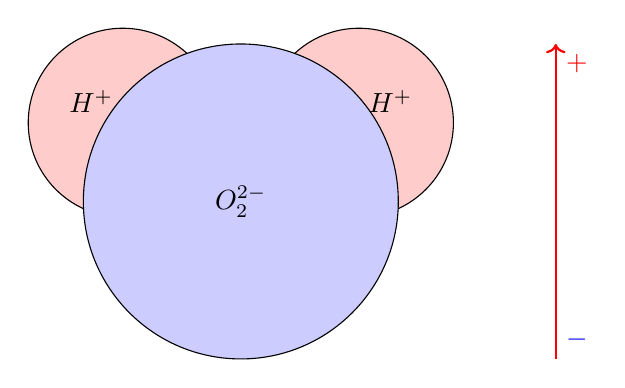
\begin{tikzpicture}
	\draw[fill=red!20] (1.5,1) circle (1.2) node [above right] {$H^+$};
	\draw[fill=red!20] (-1.5,1) circle (1.2) node [above left] {$H^+$};
	\draw[fill=blue!20] (0,0) circle (2) node {$O_2^{2-}$};
	
	\draw[<-, color=red, style=thick] (4,2) node[below right]{$\color{red}+$} to (4,-2) node[above right]{$\color{blue}-$};
\end{tikzpicture}


\newpage


\tdplotsetmaincoords{70}{100}
\tdplotsetrotatedcoords{90}{90}{90}
\begin{tikzpicture}[tdplot_main_coords]
%\begin{tikzpicture}
	\def\q{-2.3}
    \draw (0,0,0) -- ++(0,\q,0);
    
    \draw (0,0) to (0,\q) node[ground]{};

    % draw a condensor plate
    \draw[fill=lightgray] (-1.5,0,-1.5)--(-1.5,0,1.5)--(1.5,0,1.5)--(1.5,0,-1.5)--cycle;
    \draw[fill=lightgray] (1.5,0,-1.5)--(1.5,-0.2,-1.5)--(1.5,-0.2,1.5)--(1.5,0,1.5)--cycle;
    \draw[fill=lightgray] (1.5,-0.2,1.5)--(-1.5,-0.2,1.5)--(-1.5,0,1.5)--(1.5,0,1.5)--cycle;
    
    
    % dielectric
    \draw[fill=blue!20,opacity=0.7] (-1.5,-\q,1.5)--(-1.5,0,1.5)--(1.5,0,1.5)--(1.5,-\q,1.5)--cycle;
    \draw[fill=blue!20,opacity=0.7] (1.5,-\q,1.5)--(1.5,0,1.5)--(1.5,0,-1.5)--(1.5,-\q,-1.5)--cycle;
    %\draw[fill=blue!20] (1.5,0-\q,-1.5)--(1.5,\q,-1.5)--(1.5,\q,1.5)--(1.5,0-\q,1.5)--cycle;
    %\draw[fill=blue!20] (1.5,-0.2-\q,1.5)--(-1.5,-0.2-\q,1.5)--(-1.5,0-\q,1.5)--(1.5,0-\q,1.5)--cycle;
    
    \draw[<-,color=red,style=thick] (1,0,1) to (1,-\q,1);
    \draw[<-,color=red,style=thick] (1,0,-1) to (1,-\q,-1);
    \draw[<-,color=red,style=thick] (-1,0,1) to (-1,-\q,1);
    \draw[<-,color=red,style=thick] (-1,0,-1) to (-1,-\q,-1);
    
    \draw[->,style=thick] (1,0.8,0) to (1,-\q-0.8,0);
    \draw[->,style=thick] (-1,0.8,0) to (-1,-\q-0.8,0);
    
    
    %\draw[<-,color=red] (0,0,0)--++(0,-\q,0);
    %\draw[<-,color=red] (1,0,0)--++(0,-\q,0);
    %\draw[<-,color=red] (-1,0,0)--++(0,-\q,0);
    
    %\draw[<-,color=red] (0,0,1)--++(0,-\q,0);
    %\draw[<-,color=red] (1,0,1)--++(0,-\q,0);
    %\draw[<-,color=red] (-1,0,1)--++(0,-\q,0);
    
    %\draw[<-,color=red] (0,0,-1)--++(0,-\q,0);
    %\draw[<-,color=red] (1,0,-1)--++(0,-\q,0);
    %\draw[<-,color=red] (-1,0,-1)--++(0,-\q,0);

    % draw second condensor plate
    \draw[fill=lightgray] (-1.5,0-\q,-1.5)--(-1.5,0-\q,1.5)--(1.5,0-\q,1.5)--(1.5,0-\q,-1.5)--cycle;
    \draw[fill=lightgray] (1.5,0-\q,-1.5)--(1.5,-0.2-\q,-1.5)--(1.5,-0.2-\q,1.5)--(1.5,0-\q,1.5)--cycle;
    \draw[fill=lightgray] (1.5,-0.2-\q,1.5)--(-1.5,-0.2-\q,1.5)--(-1.5,0-\q,1.5)--(1.5,0-\q,1.5)--cycle;
    
    \draw (0,-\q,0)--++(0,2,0)node[above right]{$+$};
    
    
\end{tikzpicture}%




\newpage


\tdplotsetmaincoords{80}{100}
\tdplotsetrotatedcoords{90}{90}{90}
\begin{tikzpicture}[tdplot_main_coords]
%\begin{tikzpicture}
	\def\q{-3};
	\def\h{4}
	
	\draw[->,color=red, style=thick] (0,-\q/2,1.5) .. controls(0,-\q/2+0.5,0.5) .. (0,-\q/2+1,1.5);
	\draw[->,color=red, style=thick] (0,-\q/2,1.5) .. controls(0,-\q/2-0.5,0.5) .. (0,-\q/2-1,1.5);
    
    
    % dielectric
    \draw[fill=blue!20,opacity=0.5] (-1.5,-\q,1.5)--(-1.5,0,1.5)--(1.5,0,1.5)--(1.5,-\q,1.5)--cycle;
    \draw[fill=blue!20,opacity=0.5] (1.5,-\q,1.5)--(1.5,0,1.5)--(1.5,0,-1.5)--(1.5,-\q,-1.5)--cycle;
    \draw[fill=blue!20,opacity=0.5] (1.5,-\q,-1.5)--(1.5,-\q,1.5)--(-1.5,-\q,1.5)--(-1.5,-\q,-1.5)--cycle;
    %\draw[fill=blue!20] (1.5,-0.2-\q,1.5)--(-1.5,-0.2-\q,1.5)--(-1.5,0-\q,1.5)--(1.5,0-\q,1.5)--cycle;
    
    
    %\draw (0,-\q/2-1,1.5)--(0,-\q/2+1,1.5)--(0,-\q/2+1,\h)--(0,-\q/2-1,\h)--(0,-\q/2-1,1.5);  
	\draw (0,-\q/2+1,1.5)--(0,-\q/2+1,\h); 
	\draw (0,-\q/2-1,\h)--(0,-\q/2-1,1.5);   
    \draw (0,-\q/2,1.5) circle (1);
   
	  
    \draw[fill=gray!50] (0,-\q/2,1.5) circle (0.5);
    \draw[fill=gray!50] (0,-\q/2+0.5,1.5)--(0,-\q/2+0.5,\h)--(0,-\q/2-0.5,\h)--(0,-\q/2-0.5,1.5);  
    \draw[fill=gray!50] (0,-\q/2,\h) circle(0.5);    
    
    \draw (0,-\q/2,\h) circle(1);
    
    
    
    
    
	
    
    % [fill=gray!20,opacity=0.6]
    
    
	
\end{tikzpicture}




\newpage

\tdplotsetmaincoords{70}{100}
\tdplotsetrotatedcoords{90}{90}{90}
\begin{tikzpicture}[tdplot_main_coords]
%\begin{tikzpicture}
	\def\q{-2.3}
    \draw (0,0,0) -- ++(0,\q,0);
    
    \draw (0,0) to (0,-3) node[ground]{};
    
    \draw[->,color=blue!50,style=thick] (-1,-2) to (-1,-4)  to (-1, -4,-0.5) node[above left]{$I$};

    % draw a condensor plate
    \draw[fill=lightgray] (-1.5,0,-1.5)--(-1.5,0,1.5)--(1.5,0,1.5)--(1.5,0,-1.5)--cycle;
    \draw[fill=lightgray] (1.5,0,-1.5)--(1.5,-0.2,-1.5)--(1.5,-0.2,1.5)--(1.5,0,1.5)--cycle;
    \draw[fill=lightgray] (1.5,-0.2,1.5)--(-1.5,-0.2,1.5)--(-1.5,0,1.5)--(1.5,0,1.5)--cycle;
    
    \draw[<-,color=red] (0,0,0)--++(0,-\q,0);
    \draw[<-,color=red] (1,0,0)--++(0,-\q,0);
    \draw[<-,color=red] (-1,0,0)--++(0,-\q,0);
    
    \draw[<-,color=red] (0,0,1)--++(0,-\q,0);
    \draw[<-,color=red] (1,0,1)--++(0,-\q,0);
    \draw[<-,color=red] (-1,0,1)--++(0,-\q,0);
    
    \draw[<-,color=red] (0,0,-1)--++(0,-\q,0);
    \draw[<-,color=red] (1,0,-1)--++(0,-\q,0);
    \draw[<-,color=red] (-1,0,-1)--++(0,-\q,0);

    % draw second condensor plate
    \draw[fill=lightgray] (-1.5,0-\q,-1.5)--(-1.5,0-\q,1.5)--(1.5,0-\q,1.5)--(1.5,0-\q,-1.5)--cycle;
    \draw[fill=lightgray] (1.5,0-\q,-1.5)--(1.5,-0.2-\q,-1.5)--(1.5,-0.2-\q,1.5)--(1.5,0-\q,1.5)--cycle;
    \draw[fill=lightgray] (1.5,-0.2-\q,1.5)--(-1.5,-0.2-\q,1.5)--(-1.5,0-\q,1.5)--(1.5,0-\q,1.5)--cycle;
    
    \draw (0,-\q,0)--++(0,2,0)node[above right]{$+$};
    
    
\end{tikzpicture}%




\newpage


\tdplotsetrotatedcoords{90}{90}{90}
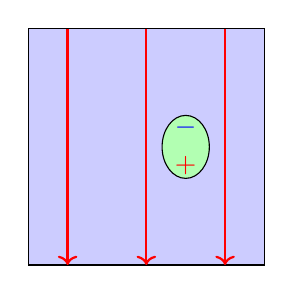
\begin{tikzpicture}
	\draw[fill=blue!20] (-1.5,-1.5)--(-1.5,1.5)--(1.5,1.5)--(1.5,-1.5)--(-1.5,-1.5);
	
	\draw[->,color=red,style=thick] (1,1.5)--(1,-1.5);
	\draw[->,color=red,style=thick] (-1,1.5)--(-1,-1.5);
	\draw[->,color=red,style=thick] (0,1.5)--(0,-1.5);
	
	\draw[fill=green!30] (0.5,0) ellipse (0.3 and 0.4) node[below]{$\color{red}+$} node[above]{$\color{blue}-$};
	
\end{tikzpicture}



\end{document}